% !TeX encoding = UTF-8

%===============================================================================
% Font options are:
%   plain (default), serif (uses Palladio), sans-serif (uses Paratype Sans)
% Layout options are:
%   article (default, no chapters), book (for longer texts, offers \chapter)
% Paragraph options are:
%   noparskip (default, no spacing between paragraphs), parskip (spaced)
\documentclass[serif,article,noparskip]{agse-thesis}

% Global parameters, replace with actual values.
\newcommand{\thesisTitle}{Untersuchung der Effizienz von RRT* bei autonomen Autos}
% -> You may use \par (but not \\) to format the title. If you do so, you'll
%    need to manually set the 'pdftitle' attribute below.
\newcommand{\studentName}{Bernd Sahre}
%===============================================================================

\hypersetup{pdftitle={\thesisTitle}}
\hypersetup{pdfauthor={\studentName}}




% Blind texts, for demonstration only, not part of the actual template
\usepackage{lipsum}
\usepackage{tabularx}

\begin{document}

\coverpage[
    student/id=4866892,
    student/mail=besahre@zedat.fu-berlin.de,
    thesis/type=Bachelorarbeit,            % optional, default: Bachelorarbeit
    thesis/group={Arbeitsgruppe Robotik},
                                           % optional, default: AGSE
    thesis/advisor={Prof. Dr. Daniel Göhring},           % optional
    thesis/examiner={Prof. Dr. Daniel Göhring},
    thesis/examiner/2={Prof. Dr. Raul Rojas}, % optional
    thesis/date=\today,                    % optional, default: \today
   %title/size=\LARGE,      % set this value to overwrite automatic font size
   %abstract/separate       % toggle this to move the abstract to its own page
]
{ % Your abstract here:
    \lipsum[1]
}

% !TeX encoding = UTF-8
\subsection*{Eidesstattliche Erklärung}

Ich versichere hiermit an Eides Statt, dass diese Arbeit von niemand anderem
als meiner Person verfasst worden ist. Alle verwendeten Hilfsmittel wie
Berichte, Bücher, Internetseiten oder ähnliches sind im Literaturverzeichnis
angegeben, Zitate aus fremden Arbeiten sind als solche kenntlich gemacht. Die
Arbeit wurde bisher in gleicher oder ähnlicher Form keiner anderen
Prüfungskommission vorgelegt und auch nicht veröffentlicht.\\

\thesisDate \\

\studentName


\cleardoublepage

\tableofcontents

\cleardoublepage

\mainmatter

% !TeX encoding = UTF-8
\section{Einleitung}
Der Traum vom autonomen Fahren reicht bis in die Antike zu den Griechen zurück, deren Gott des Feuers und der Schmiedekunst Hephaistos Androiden und selbst fahrende Automobile konstruierte. Mittlerweile ist die Forschung in diesen Bereichen von der Phantasie in die Wirklichkeit gerückt und so weit fortgeschritten, dass dieser Traum schon bald Wirklichkeit werden könnte. Zuvor müssen jedoch etliche Herausforderungen bewältigt werden. Eine davon ist, das Auto sicher durch den Straßenverkehr zu bringen. Dabei heißt sicher, dass das Auto während der Fahrt weder sich noch andere Verkehrsteilnehmer gefährdet. Neben der Sicherheit ist jedoch auch das möglichst schnelle Erreichen des Ziels wichtig, bei dem das Auto seinen Weg durch eine Umgebung mit statischen und dynamischen, das heißt sich bewegenden Hindernissen finden muss. In diesem Kontext ist noch zu erwähnen, dass dieser Weg nicht wie bei einem Navigationssystem beispielsweise von Berlin nach Hamburg führt, sondern eher von einer Straßenecke zur nächsten oder über einen Parkplatz. Dies wird durch einen Pfadplaner gewährleistet, der -informell gesprochen - aus der eigenen Position, dem Zielbereich und unter Berücksichtigung aller statischen und sich bewegenden Hindernissen einen sicheren Pfad zum Ziel findet. Dieser Pfad ist dann durch das Auto abfahrbar.\\
Um diese Aufgabe zu meistern, existieren unterschiedliche Ansätze, um dem Auto je nach Anwendungsfall bei gegebenen Ziel eine \textit{Trajektorie} vorzuschlagen. Die jeweiligen Algorithmen unterscheiden sich in Ausführungszeit, Genauigkeit, Sicherheit und berechnen unterschiedlich optimale Pfade.  \\
Das Dahlem Center for Machine Learning and Robotics untersucht maschinelles Lernen und Anwendungen intelligenter Systeme. Dazu haben sich vier Arbeitsgruppen der Freien Universität Berlin zusammengeschlossen:
\begin{itemize}
\item Intelligent Systems and Robotics (Prof. Dr. Raúl Rojas)
\item Autonomos Cars (Prof. Dr. Daniel Göhring)
\item Artifical and Collective Intelligence (Prof. Dr. Tim Landgraf)
\item Logic and automatic proofs (Christoph Benzmüller)
\end{itemize}
Ein Forschungsgebiet ist die Entwicklung und Analyse autonomer Autos. Zur oben beschriebenen Pfadplanung wird in der Arbeitsgruppe hauptsächlich das Prinzip elastischer Bänder (Time-Elastic-Bands, \citep[vgl.][]{RoeHoBe}) zur Erzeugung abfahrbarer \textit{Trajektorien} benutzt. Doch auch die Untersuchung und Analyse anderer Algorithmen ist interessant, um zu überprüfen, ob sich eine vertiefte Forschung in diesen Bereichen lohnt. \\ 
Diese Bachelorarbeit untersucht einen dieser anderen Algorithmen zur Pfadplanung, \textit{RRT*}, auf seine Tauglichkeit, über eine vorgegebene Fahrbahn mit Hindernissen eine abfahrbare, sichere und möglichst optimale \textit{Trajektorie} zu finden. 

\subsection{Aufbau und Struktur}
Nach einer kurzen Hinführung zum Thema und Vorstellung des Problems werden zuallererst die Grundlagen(\ref{sec:Grundlagen}) besprochen, um das Verständnis der nachfolgenden Kapitel zu erleichtern. Dies sind neben den grundlegenden Algorithmen auch die verwendete Hardware und Software sowie die zu berücksichtigenden Rahmenbedingungen. Im nächsten Kapitel(\ref{sec:Umsetzung})wird das Problem genauer beschrieben, anschließend folgen Analyse und Bewertung verschiedener Ansätze zur Lösung desselben. Zum Schluss (\ref{sec:Zusammenfassung}) werden in einem Fazit alle Schlussfolgerungen nochmals zusammengefasst und ein Ausblick auf weitere mögliche Forschungsmöglichkeiten gegeben. \\ 
\subsection{Problemanalyse}
\label{sec:Problemanalyse}
[TODO: Vllt. in den abstract?]
In der Bachelorarbeit von David Goedicke \citep{Goedicke18} wurden die Algorithmen $RRT^X$ und $RRT^*$ zur Berechnung eines abfahrbaren Pfades für ein Modellauto verwendet. Beide Algorithmen waren dazu in der Lage, jedoch war die Berechnungszeit zu hoch für eine Echtzeitanwendung. Dies lag unter anderem auch an den verwendeten Dubin curves und Reeds Shepp curves, die kompliziert zu berechnen sind. In dieser Arbeit wird anstelle der Reed Shepps Curves eine andere Möglichkeit untersucht, die Bewegung zwischen zwei Zuständen im Zustandsraum zu realisieren.


\subsection{Anmerkung zur Gestaltung der Arbeit}
Für die im Folgenden verwendeten personenbezogenen
Ausdrücke wurde, um die Lesbarkeit der Arbeit zu erhöhen,
ausschließlich die männliche Schreibweise gewählt. Desweiteren werden eine
Reihe von englischen Bezeichnungen und Fachwörtern verwendet, um einerseits dem
interessierten Leser das Studium der fast ausschließlich englischen
Fachliteratur zu erleichtern und andererseits bestehende Fachbegriffe nicht durch die Übersetzung zu verfälschen. Bei diesen Begriffen wird zur Unterscheidung eine kursive Schriftart verwendet.
[TODO: Wenn möglich, wurden die Quellen angegeben, bei den anderen wurde zur Definition Wikipedia verwendet.]

\subsubsection{Glossar}
\begin{tabularx}{\textwidth}{l|X}
 \textbf{Begriff}  & \textbf{Erklärung}  \\
\hline Trajektorie & Die Strecke, die dem Low-Level-Planer des Autos übergeben wird\\
Low-Level-Planer & Steuert direkt die Motoren des Autos, Lenkung und Antrieb, um eine vorgegebene Trajektorie möglichst genau abzufahren. \\
RRT & Rapidly-Exploring Random Tree \citep{Lav98}, ein Algorithmus zur Findung eines Pfades zum Ziel durch unbekanntes Gelände, wird in Kapitel \ref{RRT} noch weiter erläutert\\
RRT* & Eine verbesserte Variante des RRT, bei dem die Pfade optimiert werden \citep{KaFra10}. Asymptoptisch optimal, erläutert in Kapitel \ref{RRT*} \\
ROS & Robot Operating Systems, eine Open-Source Sammlung an Software-Bibliotheken und Werkzeugen zur Kreation von Anwendungen zur Robotik \citep{ROS}. \\
Nonholonomic Robots & Roboter, die gewissen kinematischen Einschränkungen unterworfen sind. Ein Auto zum Beispiel kann sich nicht in jede beliebige Richtung bewegen, sondern ist z.B. durch den maximalen Lenkwinkel und den Wenderadius eingeschränkt und kann nicht jeden beliebigen Punkt sofort, mit nur einem Schritt, erreichen. Im Gegensatz dazu stehen holonome Roboter, die sich in jede beliebige Richtung ohne direkte Einschränkungen bewegen können.  \\
Kinodynamic planning & Beschreibt eine Klasse von Problemen, bei der physikalische Einschränkungen wie Geschwindigkeit, Beschleunigung und Kräfte zusammen mit kinematischen Einschränkungen (z.B. Hindernisvermeidung) berücksichtigt werden müssen. \\
hochdimensionale Probleme & Probleme, bei deren Lösung nicht nur ein oder zwei, sondern sehr viele verschiedene Parameter berücksichtig werden müssen. Kinodynamic Planning befasst sich mit hochdimensionalen Problemen.\\
randomisierte Algorithmen & Algorithmen, deren Durchführung nicht determiniert ist, die also jedesmal ein etwas anderes Ergebnis zurückliefern. Der Vorteil ist, dass dies Algorithmen zwar nicht immer das bestmöglichste Ergebnis liefern, dafür aber schneller in der Ausführungszeit sind und oft einfacher zu verstehen und zu implementieren.\\
\end{tabularx} 

\begin{tabularx}{\textwidth}{l|X}
 \textbf{Begriff}  & \textbf{Erklärung}  \\
\hline 
Odroid & Einplatinencomputer am Auto mit Mehrkernprozessor. \\
Arduino Nano & Mikrocontroller am Auto zur Steuerung der Motoren und Sensoren.\\
Gyroskop & Auch Kreiselinstrument, Sensor am Auto zur Messung der Lageänderung (z.B. Ausrichtung des Autos).\\
Lidar & Light detection and ranging; Radarscanner am Auto, für Abstandsmessung zu Hindernissen.\\
Odometrie & Methode zur Schätzung von Position und Orientierung anhand der Daten des Vortriebsystems (Motoren).\\
Rewiring & Neuverknüpfung eines RRT*-Baumes \citep{KaFra10}. Die Begriffe Rewiring und Neuverknüpfung werden synomym gebraucht. Nach Hinzufügung eines Knotens K zum Baum werden Nachbarknoten überprüft, ob diese durch K besser erreichbar sind als vorher. Falls ja, wird K als Vaterknoten ausgewählt. \\
k-nearest neighbour algorithm & Algorithmus, der zu einem Punkt P die nächsten K Nachbarn bestimmt.\\
radius k-nearest neighbour & Algorithmus, der in einem Radius alle nächsten Nachbarn des Punktes P bestimmt.\\
Quaternion & 4-dimensionaler Vektor, in dem die Ausrichtung eines Objekts im Raum definiert ist.\\
\end{tabularx}
\subsection{Wichtige Quellen und deren Beitrag zum Thema}
Als wichtigste Quellen sind "Rapidly Exploring Random Trees: A new Tool for Path Planning"\citep{Lav98} von Steven LaValle und "Incremental Sampling-based Algorithms for Optimal Motion Planning" \citep{KaFra10} von Sertac Karaman und Emilio Frazzoli zu nennen. Diese führen jeweils die Algorithmen RRT und RRT* ein. Eine besonders am Anfang sehr wichtige Quelle war "Optimal Path Planning using RRT* based Approaches: A Survey and Future Directions"\citep{NoKhaHa16}, welche eine Übersicht über verschiedene Variationen und RRT* in verschiedenen Szenarien gibt. Dies hat mir bei der Orientierung und Eingrenzung des Themas sehr geholfen. [TODO subsection erscheint irgendwie sinnlos...kann man da iwie sinn hinzufügen?]\\
Nun werden wir uns den wissenschaftlichen Grundlagen der Arbeit widmen.


% !TeX encoding = UTF-8
\section{Grundlagen}
\label{sec:Grundlagen}
Dieses Kapitel führt die verwendeten Algorithmen und Berechnungen ein. Anschließend werden die Rahmenbedingungen und die verwendete Hardware und Software vorgestellt.\\
Mit dem A*-Algorithmus wurde schon in den 60er Jahren ein Werkzeug für die Pfadplanung von Robotern eingeführt \citep{astar68}. Pfadplanung bedeutet hier, dass ein Roboter mit festgelegten kinematischen Einschränkungen in einer bestimmten definierten Umgebung von einem Startzustand zu einem Zielzustand mithilfe von Steuerungseingaben gelangen kann, ohne die physikalischen Gesetze zu verletzen oder mit Hindernissen zu kollidieren. Der A*-Algorithmus löst dieses Problem unter gewissen Bedingungen, indem er in einem Graphen den kürzesten Weg zwischen zwei Knoten findet. Allerdings benötigt A* diesen Graphen zur Berechnung des Weges und ist aufgrund des hohen Speicherplatzbedürfnisses für \textit{hochdimensionale Probleme}, d.h. für Probleme mit den oben genannten kinematischen und physikalischen Einschränkungen, nicht geeignet \citep{astar68}.\\
In nachfolgender Zeit wurden \textit{randomisierte Algorithmen} entwickelt, die zwar nicht die mathematisch optimale Lösung lieferten, dafür bedeutende Geschwindigkeitsvorteile hatten. Da in der Praxis oft viele Faktoren, wie z.B. der Luftwiderstand, aufgrund der hohen Komplexität bei geringem Einfluss gar nicht berücksichtigt werden, reicht es, nur bis zu einem gewissen Grade die exakte Lösung zu liefern. \\
Diese Ansätze wurden vom \textit{randomized potential field} Algorithmus \citep{BaLa91} und dem \textit{probalistic roadmap} Algorithmus \citep{AmWu96} verfolgt. Doch auch diese waren nicht allgemein auf \textit{nonholonomic Robots} anwendbar und lösten oft nur spezifische Probleme unter ganz bestimmten Bedingungen. Der Erfolg des \textit{randomized potential field} Algorithmus beispielsweise hing stark von der Wahl einer passenden Heuristik ab \citep[vgl. Kap 3.4 in ][]{BaLa91}. Während sich bei einfachen Ausgangsbedingungen die Heuristik noch einfach finden lies, wurde dies bei komplexen, dynamischen Umgebungen mit Hindernissen und	 physikalischen und kinematischen Bedingungen zu einer großen Herausforderung. \\
1998 schließlich führte Steven LaValle den \textit{RRT}-Algorithmus ein, der die in diesem Kapitel genannten Einschränkungen umgehen sollte.

\subsection{Rapidly-Exploring Random Trees}
\label{RRT}
LaValle erkannte die die Vorteile von randomisierten Algorithmen und die \glqq erfolgreiche Einsetzung im generellen Problem der Pfadplanung\grqq{}. \citep[Kap 1][]{Lav98}. Jedoch sah er auch die Einschränkungen der vorhandenen randomisierten Algorithmen. Insbesondere störte ihn die fehlende Skalierbarkeit in komplexeren und hochdimensionalen Umgebungen, da diese Algorithmen damit nur unter gewissen Vorbedingungen effizient einsetzbar waren. Der \textit{probalistic roadmap} Algorithmus \citep{AmWu96} beispielsweise beinhaltet einen \glqq lokalen Planer\grqq, der zwar für holonomische Systeme und Roboter effiziente Ergebnisse liefert, aber bei nicht holonomischen Fahrzeugen und auf allgemeine Probleme angewendet, schwindet die Effizienz der \textit{probalistic roadmap} \citep{Lav98} .\\
Bei der Entwicklung von \textit{RRT} wurde deshalb viel Wert auf Einfachheit, Allgemeingültigkeit und damit auf Skalierbarkeit gelegt \citep[vlg. Kap 3,][]{Lav98}. Bevor wir jedoch genauer auf die Vorteile des Algorithmus eingehen und warum dieser hier gewählt wurde, folgt jetzt erstmal eine kurze Erklärung der Funktionsweise. 

Der RRT-Algorithmus baut einen Baum auf, indem zufällig gewählte Punkte unter Berücksichtigung einer Metrik verbunden werden. Der Algorithmus mit dem \textit{RRT} $T$, den Eingabeparametern Größe $K$, Metrik $M$, Bewegungsfunktion $u$ und Startzustand \verb|x_init|  funktioniert folgendermaßen:

\subsubsection{Funktionsweise der Rapidly-Exploring Random Trees}
\lstset{keywordstyle=\color{black},stepnumber=1, numbers=left}
\begin{lstlisting}
BUILD_RRT(K, M, u, x_init)
	T.init (x_init)
	for k=1 to K do
		x_rand = RANDOM_STATE();
		EXTEND(T, x_rand);
	Return T;
\end{lstlisting}
\begin{lstlisting}
EXTEND(T, x)
	x_near = NEAREST_NEIGHBOR(x, T, M);
	x_new = project(x, x_near, u);
	if (Collisionfree(x_new, x_near, u) then
		T.add_vertex(x_new);
		T.add_egde(x_near, x_new, u_new);
		Return Extended;
	else
		Return Trapped;
\end{lstlisting}

Der Baum wird anfangs mit dem Startzustand \verb|x_init| initialisiert, besteht also nur aus dem Knoten \verb|x_init|. Anschließend wird in $K$ Iterationen der Baum $T$ aufgebaut, indem mit \verb|x_rand| ein zufälliger Punkt ausgewählt und mit \verb|EXTEND(T, x_rand)| dem Baum hinzugefügt wird. \\

Die Funktion \verb|EXTEND(T, x)| ermittelt zunächst, wie in Abbildung 1 zu sehen ist, mithilfe der Metrik $M$ den nächsten Nachbar von $x$. Diese Metrik kann von einer einfachen euklidischen Distanz bis hin zur komplexen Einberechnung verschiedener kinematischer Bedingungen alles beinhalten und beeinflusst die Qualität des Baumes sowie die Berechnungsgeschwindigkeit. \\
Vom nächsten Nachbarn \verb|x_near| aus wird mit \verb|project(x,x_near,u)| ein Schritt der Länge  $\epsilon$ in Richtung x durchgeführt und an dieser Stelle der neue Knoten \verb|x_new| erzeugt. 
\begin{figure}
\centering
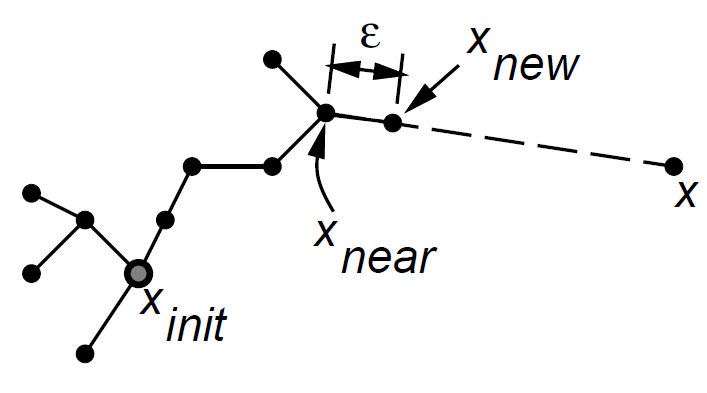
\includegraphics[scale=0.5]{Bilder/Extend.png} 
\caption{Die EXTEND Funktion \citep{Lav00} }
\end{figure} \\
Nun wird mit \verb|Collisionfree(x_new, x_near, u)| überprüft, ob \verb|x_new| oder die Bewegung $u$ zu \verb|x_new| hin mit Hindernissen kollidiert oder diesen zu Nahe kommt. Falls dies nicht der Fall ist, werden sowohl der neu entstandene Knoten \verb|x_new| als auch die Kante von \verb|x_near| zu \verb|x_new| dem Baum $T$ hinzugefügt. \\
Falls  \verb|x_new| oder die Bewegung u zu  \verb|x_new| mit Hindernissen kollidiert oder diesen zu nahe kommt, wird der Knoten  \verb|x_new| verworfen und die Funktion \verb|EXTEND(T,x)| beendet.\\

\subsubsection{Vor- und Nachteile der Rapidly-Exploring Random Trees}
Die Rapidly-Exploring Random Trees haben einige Eigenschaften, die für die Bewegungsplanung von Robotern von großem Vorteil sind, wie LaValle in  \citep[Kapitel 3 in][]{Lav98} schreibt:
\begin{enumerate}
\item Ein \textit{RRT} breitet sich sehr schnell in unerforschte Bereiche des Statusraums aus. Dadurch können Pfade schnell gefunden werden und es wird schnell eine mögliche (wenn auch nicht optimale) Lösung gefunden.
\item Die Verteilung der Knoten im Baum entspricht der Verteilung, wie diese Knoten erzeugt wurden; dies führt zu konsistentem Verhalten. Unter anderem kann dadurch das Wachstum des Baumes in eine bestimmte Richtung gesteuert werden (z.B. zum Ziel hin).
\item Ein \textit{RRT} ist probabilistisch vollständig, das heißt mit zunehmender Laufzeit konvergiert die Wahrscheinlichkeit, keinen Pfad zum Ziel zu finden, gegen null.
\item Ein \textit{RRT} ist sowohl einfach zu implementieren als auch einfach in der Analyse, was es ermöglicht, die Geschwindigkeit zu untersuchen und zu verbessern.
\item Ein \textit{RRT} ist immer mit sich selbst verbunden und das bei einer minimalen Kantenanzahl.
\item Ein \textit{RRT} kann als Pfadplanungsmodul interpretiert werden, was die Kombination mit anderen Werkzeugen zur Bewegungsplanung möglich macht.
\end{enumerate}
Leider existieren neben den oben genannten Vorteilen auch etliche Nachteile. Eines der größten ist, dass ein \textit{RRT} nicht den optimalen Pfad zurückliefert, da einmal gesetzte Knoten ihren Vaterknoten nicht mehr ändern können. Dadurch kann, auch wenn durch Neuverknüpfung eine bessere Knotenfolge vom Start zum Ziel bestehen würde, diese nicht erstellt werden. Außerdem bereichern Knoten, die innerhalb des bereits bestehenden Baumes hinzugefügt werden, selten den RRT.\\

\begin{figure}[htb]
    \centering
 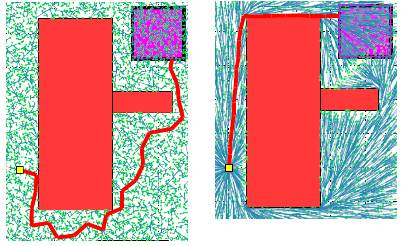
\includegraphics[scale=1]{Bilder/RRT_RRT_star.png} 
 \caption{RRT(links) und RRT* (rechts) mit jeweils 20.000 Knoten}
      
\end{figure}

Deshalb wurde von Sertac Karaman und Emilio Frazzoli aufbauend auf \textit{RRTs} der Algorithmus\textit{ RRT*} eingeführt, welcher diesen Nachteil ausgleicht(siehe Abbildung 2).
\subsection{Rapidly-Exploring Random Tree Star}
\label{RRT*}
Im Gegensatz zu einem \textit{RRT} führt ein \textit{RRT*} die zwei folgenden Neuerungen ein:
\begin{enumerate}
\item Auswahl eines passenden Vaterknotens bei Hinzufügen des Knotens zum Baum
\item Neuverknüpfung des Baumes
\end{enumerate}
Diese Neuerungen resultieren in einer veränderten \verb|EXTEND(T,x)| Funktion, siehe \citep{KaFra10}.
\subsubsection{Funktionsweise eines Rapidly-Exploring Random Tree Star}
\begin{lstlisting}
EXTEND(T,x)
	x_nearest = NEAREST_NEIGHBORS(x, T, M);
	x_new = project(x, x_nearest, u);
	if (Collisionfree(x_new, x_near, u) then
		T.add_vertex(x_new);
		x_min= x_nearest;
		c_min = x_nearest.cost + cost(x_nearest, x_new);
		X_NEAR = NEAR_NEIGHBORS(x, T, r);
		foreach x_near in X_NEAR do
			if Collisionfree(x_near, x_new) && x_near.cost + cost(x_near, x_new) < c_min then
				x_min = x_near;
				c_min = x_near.cost + cost(x_near, x_new);
		T.add_egde(x_min, x_new);
		foreach x_near in X_NEAR do
			if Collsionfree(x_new, x_near) && x_new.cost + cost(x_new, x_near) < x_near.cost then
				T.del_edge(x_near_parent, x_near);
				T.add_edge(x_new, x_near);
		Return Extended;
	else
		Return Trapped;
\end{lstlisting}

Während, wie beim Erstellen eines \textit{RRT}, auch bei \textit{RRT*} zuerst der nächste Nachbar als Vaterknoten festgelegt wird, folgt daraufhin ein Speichern der nächsten Nachbarn von \verb|x_new| in einem gewissen Radius $r$ in der Liste \verb|X_NEAR|. 
Es wird \verb|x_min| als der Abstand zum nächsten Knoten gesetzt. Die Funktion \verb|x_nearest.cost| liefert die Kosten, um vom Startknoten zu \verb|x_nearest| zu kommen, zurück, während die Funktion \verb|cost(x_nearest, x_new)| die Kosten des Pfades von \verb|x_nearest| zu \verb|x_new| berechnet. Als vorläufiger Startwert beinhaltet \verb|c_min| demnach die Kosten, um vom Startknoten aus zu \verb|x_new| zu kommen. \\
Die Liste \verb|X_NEAR| wird auf den besten Vaterknoten, also den mit den geringsten Kosten für \verb|x_new|, überprüft. Dieser beste gefundene Nachbar wird für \verb|x_new| als Vaterknoten gesetzt, also eine Kante zwischen \verb|x_new| und \verb|x_near| gezogen. \\
\label{sec:rewiring}
Nachdem so ein Pfad vom Vaterknoten zu \verb|x_new| gebildet wurde, wird der Baum neu verknüpft. Bei jedem Knoten innerhalb des Radius von \verb|x_new| wird überprüft, ob die Kosten mit \verb|x_new| als Vaterknoten geringer werden. Wo immer dies der Fall ist, wird \verb|x_new| als Vaterknoten gesetzt.
\subsubsection{Vor- und Nachteile der Rapidly-Exploring Random Trees Star}
\label{sec:rrt*}
Eine Verbesserung zu einem \textit{RRT} ist, dass nicht der nächste Nachbar als Vaterknoten gesetzt wird, sondern der mit den besten Kosten. Je nach Wahl des Radius $r$ und Güte der Kostenfunktion kann hier einiges an \glqq Umweg\grqq{} gespart werden. \\
Der Hauptunterschied ist jedoch die Neuverknüpfung bereits bestehender Knoten über \verb|x_new|. Ein Nachteil des \textit{RRTs} ist, dass Knoten, die aus bereits gut mit Knoten gefüllten Regionen neu hinzugefügt wurden, wenig neues beitragen, also weder neue Regionen entdecken, noch bestehende Pfade verbessern. Dies ändert sich nun, denn jeder von Knoten umgebene, neu hinzugefügte Knoten verbessert die Kosten aller Knoten, die durch \verb|x_new| besser erreichbar sind. Das führt dann sogar soweit, dass ein \textit{RRT*} asymptotisch optimal ist, d.h. bei genügend langer Laufzeit der Pfad zum Optimum konvergiert. Jeder Knoten hilft entweder, den Baum zu expandieren oder sorgt für bessere Pfade innerhalb des Baumes (\citep[vgl. Kapitel 5 in][]{KaFra10}). Je nach Art der Kostenfunktion und dem Samplen neuer Knoten kann der RRT* auch mit bestimmten Eigenschaften ausgestattet werden, z.B. präferiertes Wachsen in bestimmte Richtungen.

Als nächstes werden die Hardware und das verwendete Framework ROS - Robot Operating Systems - vorgestellt. \\
Anschließend werden potentielle Metriken und Datenstrukturen präsentiert.
Bevor wir uns dann den notwendigen Anpassungen des \textit{RRT*}-Algorithmus widmen können, werden die kinematischen und physikalischen Beschränkungen des Autos analysiert.
\subsection{Hardwareausstattung der Autos}
Das Dahlem Center for Machine Learning and Robotics arbeitet mittlerweile mit dem Modellfahrzeug AutoNOMOS Mini v3 (1:10).
\begin{figure}
\centering
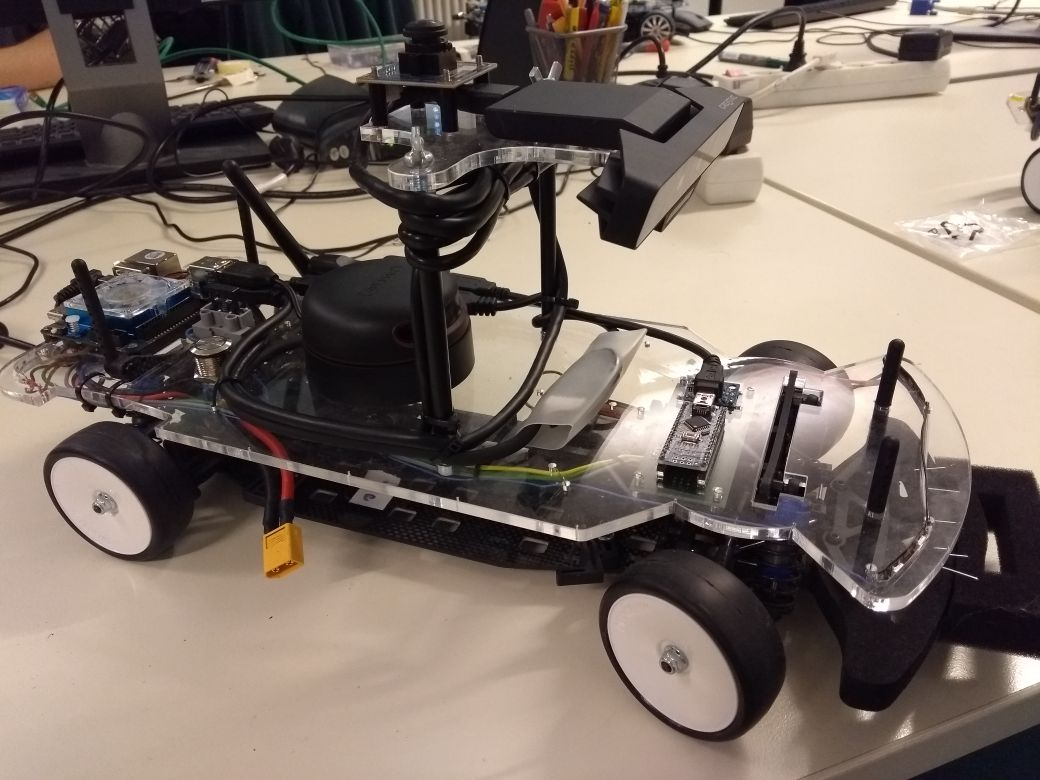
\includegraphics[scale=0.3]{Bilder/car.jpg} 
\caption{Autonoms Mini v3 (1:10)}
\end{figure}
 Der Hauptcomputer des Autos ist ein \textit{Odroid}(XU4 64GB) mit Ubuntu Linux als Betriebssystem und ROS (Robot Operation Systems) zur Steuerung \citep{fubAuto}.\\
\begin{figure}
\centering
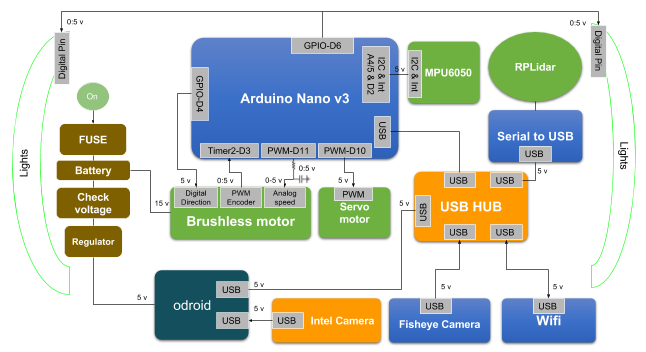
\includegraphics[scale=0.8]{Bilder/AutoNOMOS_mini_v3.png} 
\caption{Überblick über die Module des AutoNOMOS Mini v3}
\end{figure}
Motorisiert ist das Auto mit einem bürstenlosen DC-Servomotor FAULHABER 2232. Die Lenkung wird von dem Servomotor HS-645-MG übernommen; beide Motoren werden mithilfe einer \textit{Arduino Nano} Platine gesteuert. \\
Zur Wahrnehmung der Umgebung besitzt das AutoNOMOS Mini v3 mit dem RPLIDAR A2 360 einen rotierenden Laserscanner, der in der Lage ist, die Umgebung des Autos auf Hindernisse zu überprüfen. Als Rückgabewert liefert der RPLIDAR pro Gradwinkel einen Wert in Metern, wie weit das nächste Hindernis in dieser Richtung entfernt ist, insgesamt also 360 Werte. \\
Auf dem oberen Teil des Autos befestigt ist das \textit{Kinect-type stereoscopic system} (Intel RealSense SR300), welches eine Wolke aus 3D Punkten liefert, die dazu benutzt werden kann, Hindernisse zu erkennen. Außerdem kann die Kamera des \textit{Kinect-type} Sensors dazu benutzt werden, Fahrbahnmarkierungen und Objekte direkt vor dem Auto zu lokalisieren.\\
Der letzte äußere Sensor, auch am oberen Teil des Autos angebracht, ist die Fischaugen-Kamera. Diese zeigt nach oben zur Decke, und kann dazu benutzt werden bestimmte markante, feststehende Objekte zu lokalisieren, damit das AutoNOMOS Mini v3 sich auch innerhalb von Räumen orientieren kann. Dazu kann eine GPS Navigationseinheit simuliert werden, indem die an der Decke angebrachten vier Lampen in unterschiedlichen Farben leuchten.
Die Sensoren sind entweder via USB 3.0 an der Hauptplatine oder direkt am \textit{Odroid} angeschlossen. Dies ist in Abblidung 4 zu sehen.\\
An inneren Sensoren besitzt das AutoNOMOS Mini v3 eine MPU6050, die einen Beschleunigungssensor und ein \textit{Gyroskop} enthält. Mithilfe dieser MPU kann das AutoNOMOS Mini v3 seine Orientierung, seine Richtung im Raum bestimmen. Außerdem können Messungen zur \textit{Odometrie} ergänzt werden.\\
Das AutoNOMOS Mini v3 wird über eine 14,8 V Batterie mit Energie versorgt.

\subsection{Software: ROS - Robot Operating Systems}
ROS stellt Bibliotheken und Werkzeuge zur Verfügung, die Software-Entwicklern helfen sollen, Robotik-Anwendungen zu kreieren \citep{ROS}. Unter anderem beinhaltet ROS Gerätetreiber, Bibliotheken, Visualisierungswerkzeuge, Paketmanagement und vieles mehr. ROS ist quelloffen und unter der BSD Lizenz verfügbar.\\

Mithilfe von ROS können ausführbare Programme, auch Knoten genannt, erzeugt werden, die über so genannte \textit{Topics} kommunizieren können. Dies passiert über einen anonymisierten Publisher/Subscriber Mechanismus, das heißt Daten generierende Knoten können auf relevanten \textit{Topics} Nachrichten senden und Knoten, die Daten benötigen, können von relevanten \textit{Topics} Nachrichten empfangen. \\
Für jedes \textit{Topic} ist dabei auch die Nachrichtenart definiert, die für dieses \textit{Topic} veröffentlicht und von diesem \textit{Topic} empfangen werden. Diese kann neben simplen Datentypen auch aus komplexen, selbst definierten Datenstrukturen bestehen. Dabei wird nur dieser eine, vorher festgelegte Datentyp der Nachricht vom \textit{Topic} akzeptiert.
\textit{Topics} stellen nur eine unidirektionale Verbindung zur Verfügung. Für die Abwicklung von zum Beispiel Remote Procedure Calls sind sogenannte Services zuständig. Diese ermöglichen eine Antwort auf eine bestimmte Anfrage nach dem Client Server Prinzip zurückzusenden.
\subsection{Schnittstellen und Einbettung zu bereits vorhandene Knoten}
Das Dahlem Center for Machine Learning and Robotics entwickelte ROS-Pakete für die Steuerung ihrer autonomer Fahrzeuge. Diese Pakete und daraus resultierenden ROS-Nodes können dazu genutzt werden, den von mir entwickelten RRT*-Pfadplaner möglichst gut einzubetten. So kann durch das visuelle indoor GPS die Position des Autos bestimmt werden, die der Pfadplaner für seine Berechnungen braucht. Die resultierende \textit{Trajektorie}, die der Pfadplaner entwickelt, wird dem Low-Level-Planer übergeben, der diese \textit{Trajektorie} in Motorbefehle, also Beschleunigungen und Lenkungen, umsetzt. 
\subsubsection{Bestimmung der Odometrie und visuelles GPS}
Zur Ausführung des Algorithmus gehört, dass das Auto sich selbst lokalisieren kann und seine eigene Startposition feststellen kann. Diese wird mit der aktuellen Ausrichtung des Autos dazu benutzt, den Startpunkt für den Algorithmus zu setzen. \\
Das Dahlem Center for Machine Learning and Robotics hat dafür zwei verschiedene Varianten entwickelt, die sich kombiniert gegenseitig ergänzen können. \\
\begin{enumerate}
\item Odometrie \\
Anhand des Lenkwinkels und der Motordrehgeschwindigkeit kann die erwartete Position, Geschwindigkeit und Beschleunigung berechnet werden. Mit dem im Auto verbauten Gyroskop werden Lageänderungen entlang jeder Achse gemessen. Aufgrund mechanischer Beschränkungen und Ungenauigkeiten sind Messungen mithilfe der Odometrie nie ganz exakt und somit kann eine so bestimmte Position mit der Zeit von der tatsächlichen Position abweichen.
\item Visuelles GPS\\
Da es innerhalb von Gebäuden Schwierigkeiten mit der genauen Positionsbestimmung via GPS gibt, wurde mithilfe von vier Lampen, die an der Decke angebracht wurden, ein visuelles GPS simuliert. Diese vier Lampen leuchten in unterschiedlichen, gut erkennbaren Farben und werden mit der Fischaugenkamera, die zur Decke ausgerichtet ist, erfasst. Anhand der Lage der Lampen zueinander und wie die Fischaugenkamera diese sieht, kann die Position des Autos bestimmt werden.\\
Dazu muss jedoch gesagt werden, dass das eindeutige Erkennen der Lampen nur unter guten Bedingungen (Lichtverhältnisse, alle 4 Lampen im Bild) möglich ist. 
\end{enumerate}

\subsubsection{Low-Level-Planer}
Das Dahlem Center for Machine Learning and Robotics entwickelte den Low-Level-Planer "fub controller", der für die Steuerung der Motoren zuständig ist.
Dieser Planer lauscht auf das \textit{Topic} \verb|"planned_path"|. Auf \verb|"planned_path"| kann eine \textit{Trajektorie} publiziert werden, die dann mithilfe des Low-Level-Planers vom Auto abgefahren wird. Dabei kümmert sich dieser Planer allerdings nicht um etwagige Hindernisse, die mit dem Auto kollidieren könnten, sondern fährt nur die Trajektorie ab. Somit muss der Pfadplaner selbst alle Kollisionen mit Hindernissen ausschließen. \\
Das Format der \textit{Trajektorie} wurde von der Arbeitsgruppe der FU Berlin definiert und besteht aus
\begin{itemize}
\item \verb|std_msgs/Header|: Hier wird die aktuelle Zeit gespeichert.
\item \verb|string child_frame_id|: Koordinatensystem, in dem die Trajektorie eingebettet wird.
\item \verb|fub_trajectory_msgs/TrajectoryPoint[] trajectory|: Eine Liste aus Trajektorie-Punkten.
\end{itemize}
Ein Trajektorien-Punkt symbolisiert einen abzufahrenden Knotenpunkt und besteht wiederum aus
\begin{itemize}
\item \verb|geometry_msgs/Pose pose|: Hier sind Position und Orientierung des Autos gespeichert.
\item \verb|geometry_msgs/Twist velocity|: Hier wird die Geschwindigkeit des Autos an diesem Punkt gespeichert.
\item \verb|geometry_msgs/Twist acceleration|: Hier wird die Beschleunigung des Autos an diesem Punkt gespeichert.
\end{itemize}
Die Position wird in x-Position und y-Position ausgehend von einer Ecke des Raumes angegeben. Die Orientierung wird durch ein \textit{Quaternion} dargestellt, bei dem durch vier Werte die Drehung in jeder Richtung des Raumes genau bestimmt ist. Allerdings genügt uns die Drehung um die z-Achse, also die Drehrichtung über die Vertikalachse, weshalb dieses Quaternion in einen Winkel, der sogenannten Gierung( engl. \textit{yaw}), umgerechnet wird.
\\

\subsection{Datenstruktur}
Um die Anwendung in Echtzeit zu nutzen, muss die Geschwindigkeit des RRT* Algorithmus sehr hoch sein. Der gesamte Algorithmus, bestehend aus Aufbau des Baumes, Rewiring, dem Finden einer gültigen Trajektorie vom Start zum Ziel und Vermeiden von Hindernissen sollte nicht mehr als 250 Millisekunden brauchen. Dadurch wird gewährleistet, dass auch sich bewegende Hindernisse stets erkannt werden und der Pfad des Autos gültig bleibt. \\
RRT* erzeugt n Punkte. Jeder dieser Punkte sucht zuerst seinen nächsten Nachbarn, dann wird der Punkt an den Baum projiziert und dem Baum hinzugefügt. Am Ende wird der Baum neu verknüpft. \\
Unter der Voraussetzung, dass die Suche des nächsten Nachbarn in der Zeit O(log n) zu bewerkstelligen ist, hat RRT* eine Laufzeit von O(n log n). Dies ist jedoch nur durch die Wahl einer passenden Datenstruktur zu erreichen, die \textit{k-nearest neighbour} Suche und \textit{radius k-nearest neighbour} in O(log n) durchführen können.\\
Es existieren bereits viele wissenschaftliche Untersuchungen und auch empfohlene Datenstrukturen, wie zum Beispiel k-d-Bäume \citep{Bentley75}. Leider benötigt der RRT* Algorithmus eine dynamische Datenstruktur, da Punkte erst nach und nach hinzugefügt werden. Das Hinzufügen eines Punktes muss somit auch in logarithmischer Zeit gewährleistet sein. 

Aufgrund fehlender Implementierungen und Mangel an Zeit zum Erstellungszeitraum dieser Arbeit konnte eine solche Datenstruktur nicht mehr im Zusammenhang mit dieser Arbeit implementiert werden. Der alternative Versuch, mit Hilfe der Bibliothek nanoflann \citep{blanco2014nanoflann} die Knoten in einen k-d-Baum zu verwenden, scheiterte an der fehlenden dynamischen Unterstützung.

Deshalb wurde versucht, eine einfachere Datenstruktur mit den ersehnten Eigenschaften zu entwerfen. Dazu wurde ein einfaches Gitter implementiert, deren Achsen die x- und y-Werte des einzufügenden Punktes repräsentierten. Dadurch fallen Punkte, die nah beieinander sind, in die gleiche oder benachbarte Zellen. Je nach Wahl der Größe der Zellen müssen nur die Knoten der Zelle selbst und der Nachbarzellen überprüft werden. Ein weiterer Vorteil des Gitters ist das schnelle Einfügen eines Knotens: Dadurch dass das Gitter statisch bleibt, können Arrays als Rahmen gewählt werden und die Laufzeit zum Einfügen von Knoten liegt bei O(1).

Im optimalen Fall muss bei der \textit{k-nearest neighbour} Suche nur die Zelle, worin der Knoten liegt, sowie alle acht angrenzenden Zellen untersucht werden. Solange sich allerdings nur sehr wenige Knoten im Gitter befinden, muss unter Umständen das gesamte Gitter nach Nachbarn abgesucht werden, was die Laufzeit stark verschlechtert. Innerhalb einer Zelle sind die Knoten in einer Liste gespeichert. Sollten sehr viele Knoten in eine Zelle fallen, dauert das Durchsuchen dieser Zelle sehr lange. Wird also die Zellgröße groß gewählt, dauert das Durchsuchen einer Zelle lange, wird sie klein gewählt, müssen zu viele Zellen durchsucht werden. 

Aufgrund einer zu hohen Laufzeit und Fehleranfälligkeit wurde das Gitter verworfen und zur Speicherung der Knoten eine einfache Liste gewählt. Dadurch hat der Algorithmus zwar eine Laufzeit von O($n^2$), dafür waren die Fehleranfälligkeit und der zeitliche Implementierungsaufwand nicht so hoch. \\
\subsection{Sonstige verwendete Software}
Anfangs wurde in der Programmiersprache Python programmiert. Zur Verbesserung der Geschwindigkeit wurde jedoch schnell zu C++ gewechselt. Als Entwicklungsumgebung wurde Eclipse mit dem CDT-Plugin gewählt. \\
Zur Berechnung der Vektorarithmetik wurde die C++ Headerbibliothek Eigen3 verwendet.

Nachdem die notwendige Infrastruktur und verwendete Software erläutert wurde, folgt eine kurze Betrachtung der kinematischen und physikalischen Einschränkungen, denen das AutoNOMOS Mini v3 unterworfen ist. Anschließend wird sich im Folgenden dem Kernstück der Arbeit, dem eigentlichen RRT*-Pfadplaner, gewidmet.
\subsection{Kinematische und physikalische Einschränkungen}
Im Gegensatz zu holonomischen Fahrzeugen, die sich ohne Einschränkungen in alle Richtungen des Raumes bewegen können, sind die möglichen Pfade eines nicht holonomischen Fahrzeug wie ein Auto nicht so einfach zu berechnen. Deshalb stellen wir zuerst ein mathematisches Modell des Autos auf und definieren die Randbedingungen, unter denen es agiert.
Die mathematischen Definitionen der Randbedingungen und des Autos sind in der Bachelorarbeit von David Gödicke \citep{Goedicke18} gut beschrieben und werden hier übersetzt übernommen. \\
\subsubsection{Randbedingungen}
Die Position des Autos bezieht sich auf den Mittelpunkt zwischen den Hinterrädern mit den Koordinaten x und y. Der Winkel $\theta \in S,  S=[0,2\pi]$ steht für die Ausrichtung des Autos, der Winkel $\phi \in S$ für die Ausrichtung der Räder (=Lenkwinkel). Wir nehmen an, dass das Auto sich auf einer flachen Ebene bewegt. Somit ist der Arbeitsraum definiert durch $C =  \mathbb{R \times S}$. Ein Zustand des Autos wird beschrieben durch $q \in C = (x,y,\theta)$.\\
Zur Vereinfachung der Rechnungen wird angenommen, dass die Räder bei Bedarf sich sofort, ohne Zeitverlust, in die gewünschte Position begeben. Da der Lenkwinkel keinen Einfluss auf den Momentanzustand des Autos hat, wird dieser in der Zustandsbeschreibung nicht aufgeführt. Zusätzlich kommt noch hinzu, dass das Auto zur Testzwecken bestimmte Geschwindigkeiten nicht überschreiten darf, sodass der minimale Kurvenradius nur durch den Lenkwinkel beschränkt ist und nicht auch noch zusätzlich durch die Geschwindigkeit. \\
Die durch den Algorithmus berechnete Trajektorie führt von der Startposition des Autos (Startknoten) über eine Anzahl von Knoten bis zu einem Zielknoten im Zielbereich. Jeder Knoten K ist definiert mit $K= (x,y,\theta, c, V)$. X und y sind die Koordinaten des Knotens, $\theta$ die Ausrichtung, die das Auto in diesem Knoten hätte. C sind die durch eine Kostenfunktion \ref{sec:Kosten} berechneten Kosten, um vom Startzustand zu diesem Knoten zu gelangen und V ist der Vaterknoten. 

\subsubsection{Einschränkungen durch das Auto}
Der Zustand des Autos kann durch Beschleunigung verändert werden. Ein negatives Beschleunigen entsteht beim Bremsen oder Rückwärtsfahren. Zusätzlich zu dieser einen Möglichkeit, den Zustand des Autos zu ändern, kann das Auto das Resultat der Beschleunigung ändern, indem der Lenkwinkel angepasst wird. Dieser reicht von $\phi_{max}$ bis $-\phi_{max}$, den maximalen Lenkwinkeln des Autos.
Je nach Lenkwinkel $i_{\phi}$, Geschwindigkeit $i_g$ und Anfangsausrichtung des Autos $\theta$ ändern sich verschiedene Parameter des Zustandes $q(x,y, \theta) $: \\
\begin{center}
$ \dot{x} = i_g cos \phi $ \\
$ \dot{y} = i_g sin \phi$ \\
$ \dot{{\theta}} = \frac{i_g}{L} tan (i_{\phi}) $
\end{center}
L ist hierbei der Radstand, also der Abstand zwischen der Vorder- und der Hinterachse. \\


% !TeX encoding = UTF-8
\section{Umsetzung}
\label{sec:Umsetzung}
Es gibt unterschiedliche Vorgehensweisen, einen RRT* zu bauen und neu zu verknüpfen. Besondere Bedeutung hat dabei, wie neu erzeugte Knoten dem Baum hinzugefügt werden. David Gödicke benutzte in seiner Bachelorarbeit zum Erreichen zweier Punkte innerhalb des Baumes Dubin curves \citep{Dubin61} beziehungsweise Reed Sheep curves \citep{reeds1990optimal}, sodass der neu hinzugefügte Knoten stets durch seinen Vater erreichbar war \citep{Goedicke18}. Leider war die Berechnung dadurch insgesamt zu aufwändig und langsam, was für Echtzeit-Szenarien im Straßenverkehr ein hartes Ausschlusskriterium ist, weshalb Goedicke diesen Ansatz nicht empfehlen konnte \citep[vergleiche][Kapitel 7]{Goedicke18}. \\
Daher entschloss ich mich, Varianten von RRT* zu untersuchen, bei denen das Auto direkt von Knoten zu Knoten fährt. Dadurch benötigt es nur eine Lenkeinstellung zwischen zwei Knoten und die Berechnung wird einfacher.\\
\begin{figure}
	\label{fig:reachable}
	\centering
	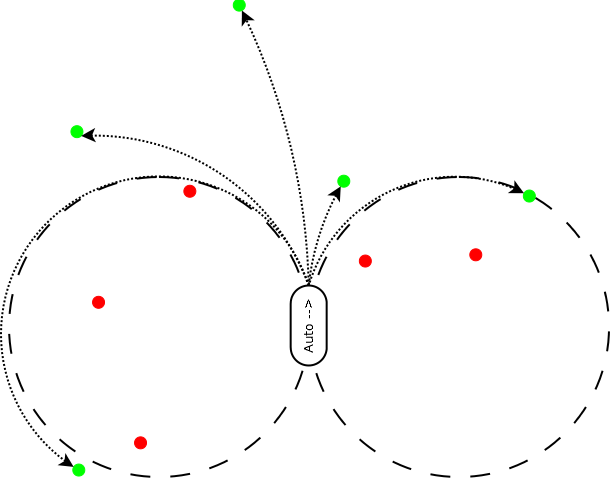
\includegraphics[scale=0.6]{Bilder/Erreichbarkeit_Punkte.png}
	\caption{Erreichbare und nicht erreichbare Punkte vom Auto aus}
\end{figure}
\subsection{Übersicht}
\label{sec:uebersicht}
Hier werden vier verschiedene Ansätze vorgestellt, mit deren Hilfe das Auto mit dem RRT* Algorithmus von der Startposition in den Zielbereich kommt.
\begin{enumerate}
\item Erster Ansatz: Nicht erreichbare Knoten werden dem Baum nicht hinzugefügt. Kostenfunktion berücksichtigt Lenkänderungen. Rewiring findet Rekursiv statt.
\item Zweiter Ansatz: Alle Knoten sind erreichbar, aber nur außerhalb der Wendekreise. Kostenfunktion berücksichtigt Lenkänderungen. [TODO: Rewiring?]
\item Dritter Ansatz: RRT* ohne Einschränkungen durchgeführt, das heißt alle Knoten sind gültig. Am Ende wird ein Pfad vom Ziel zum Startknoten erstellt, der abfahrbar ist.
\item Vierter Ansatz: Nicht erreichbare Knoten werden dem Baum nicht hinzugefügt. Kostenfunktion berücksichtigt Lenkänderungen. Rewiring wird nur bei dem Knoten mit der besten Kostenersparnis durchgeführt.
\end{enumerate}
Dabei müssen diese Ansätze folgende Bedingungen erfüllen: \\
\begin{enumerate}
\item Garantie der Abfahrbarkeit: Das Auto muss in der Lage sein, der berechneten Trajektorie zu folgen. Da das Auto die Punkte innerhalb der Wendekreise nicht erreichen kann(siehe \ref{fig:reachable}), muss sichergestellt werden dass diese Punkte nicht als Kindknoten gewählt werden können.
\item Geringe Kosten: Es muss nicht der optimale Pfad gefunden werden, aber er sollte zumindest asymptotisch optimal sein. 
\item Niedrige Berechnungsdauer: Da der Algorithmus mehrmals pro Sekunde ausgeführt werden soll, sind Ausführzeiten über 250 Millisekunden nicht tolerierbar. Bei Messungen der Ausführzeit muss jedoch auch die Wahl der Datenstruktur, Metrik und die Art der Implementierung berücksichtigt werden, da diese zusätzlich die Laufzeit verändern können.
\end{enumerate}
Die vier Ansätze werden anhand der obigen Kriterien untersucht und bewertet.

\subsection{Erster Ansatz}
Ziel ist es hier, nur Knoten hinzuzufügen, die vom jeweiligen Vaterknoten auch erreichbar sind. Um eine bessere Laufzeit zu erreichen, wurde schon bei der Suche des nächsten Nachbarn eine Vorauswahl getroffen und ein Großteil der nicht vom Baum erreichbare Knoten aussortiert. Bei der tatsächlichen Bestimmung des Vaterknotens werden dann mithilfe eines genaueren Mechanismus nur Knoten berücksichtigt, von denen aus der neu hinzugefügte Knoten erreicht werden kann. \\
Nach dem Setzen des Vaterknotens werden mit einer Kostenfunktion die Kosten berechnet, um diesen Knoten zu erreichen. Zum Schluss findet das Rewiring, das neu verknüpfen des Baumes, statt.
\subsubsection{Vorauswahl}
\label{sec:Vorauswahl}
Diese beinhaltete, bei der Erstellung des RRT* vom Auto nicht erreichbare Knoten gar nicht erst zuzulassen. Das Auto sollte also von einem Knoten zum nächsten mit nur einer Lenkeinstellung direkt fahren können. Dies sollte die Berechnungszeit stark verringern. \\
Zum Ausschluss der Knoten verwendete ich zuerst eine Heuristik: Ein nächster Nachbar N für einen neu hinzugefügten Knoten K kam nur dann in Frage, falls dieser den neu hinzugefügten Knoten K auch erreichen konnte. Dazu wurde die Ausrichtung des Autos im potenziellen Elternknoten N mit dem Richtungsvektor zwischen den beiden Knoten verglichen. Somit war K gültig, falls der Winkel zwischen der Ausrichtung von N und dem direktem Weg zum Knoten K (Richtungsvektor) einen bestimmten Wert $\gamma$ nicht überschritt.
\begin{figure}
\centering
\label{fig:fig4}
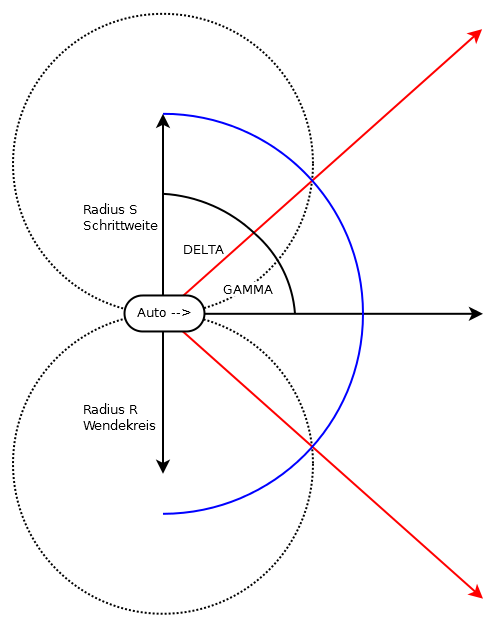
\includegraphics[scale=0.6]{Bilder/AusrichtungGrob.png} 
\caption{Bedeutung der Schrittweite und Radius für den Winkel Gamma}
\end{figure}
 $\gamma$ direkt zu berechnen war nicht ohne weiteres möglich, doch mit Hilfe des Kosinussatzes konnte der Winkel $\delta$ (siehe Abbildung ~\ref{fig:fig4}) berechnet werden. Dieser berechnet sich aus dem Radius $R$ des Wendekreises des Autos und der verwendeten Schrittweite, also dem maximalen Abstand zwischen zwei Knoten. \\
Der Knoten K wurde im ersten Schritt als gültig erkannt, wenn für die Differenz zum Winkel des Elternknoten galt: 
\begin{center}
$diff(K,N) <\gamma$ \\
$\gamma = 90^{\circ} - \delta$  \\
$\delta = arccos (\frac{Schrittweite}{2 \dot R})$  \\
\end{center}

Alle Knoten außerhalb dieses Winkels würden bei der Projektion im Wendekreis des Autos landen, wie in Abbildung \ref{fig:fig5} zu sehen. Diese Knoten(rot) wurden verworfen.\\
\subsubsection{Auswahl des Vaterknotens}
\label{sec:Auswahl}
Als nächster Schritt wird, wie in Kapitel \ref{RRT*} geschildert, der Knoten K an den nächsten (gültigen) Nachbarn N projiziert und der Vaterknoten bestimmt. Sollte der Knoten näher am Vaterknoten dran sein, als die Schrittweite ist, wird der Knoten nicht projiziert, da sonst alle Knoten zu ihrem Vaterknoten den gleichen Abstand hätten und bestimmte Bereiche somit nicht auf optimalen Weg erreichbar wären. Da innerhalb der Schrittweite durch den maximalen Lenkwinkel des Autos selbst die Knoten, die vom Winkel her gültig sind, nicht erreichbar sein können, ist eine zusätzliche Überprüfung für diese Knoten notwendig (siehe \ref{fig:fig5}). \\
Da der maximale Lenkwinkel eines Autos vorgegeben ist, hängt also die Erreichbarkeit des Knotens allein von der Schrittweite ab. Mit dieser kann auch vorgegeben werden, um wie viel Grad sich die Ausrichtung des Autos bei einem Schritt ändern darf und ob beispielsweise Kehren erlaubt sind. Dabei muss jedoch beachtet werden: Bei einer zu kleinen Schrittweite werden viele Knoten verworfen und es werden kaum enge Kurven möglich sein. Bei einer zu großen Schrittweite werden sehr kurvige Trajektorien entstehen, sodass z.B. Hinderniserkennung nicht mehr so einfach ist.
\begin{figure}
\centering
\label{fig:fig5}
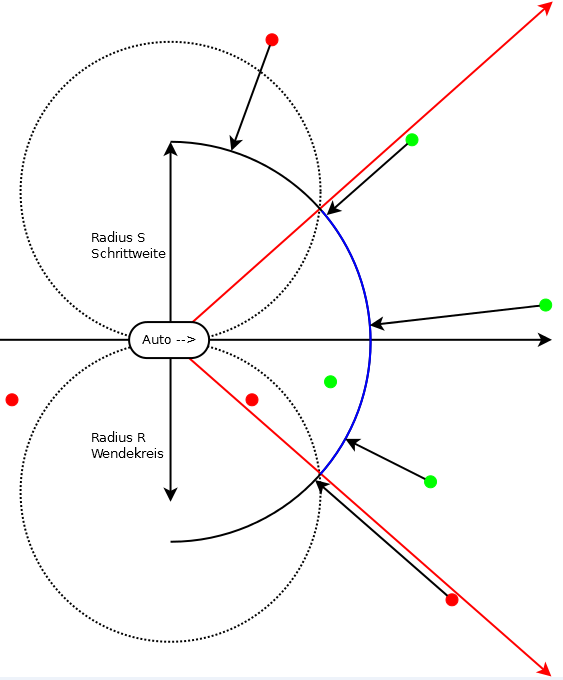
\includegraphics[scale=0.6]{Bilder/Projektion_der_Punkte.png} 
\caption{Projektion der Punkte auf Schrittweite}
\end{figure}
\subsubsection{Bestimmung des Vaterknotens}
Nachdem der Knoten an seinen nächsten Nachbarn projiziert wurde, wird nun aus allen nächsten Nachbarn innerhalb eines Radius R der mit den besten Kosten gewählt. Im Verfahren zur Bestimmung des nächsten Nachbarn, siehe \ref{sec:Vorauswahl}, wurden nicht beachtet, dass der neue Knoten innerhalb der Wendekreise des Autos liegen könnte. Es ist dem Auto aber nicht möglich, vom Vaterknoten N zum Knoten K zu fahren, wenn K im Wendekreis des Autos liegt. \\
Für jeden Knoten im Radius R wird geprüft, ob dieser Knoten unseren neuen Knoten K erreichen kann. Das wird ausgerechnet, indem vom potentiellen Vaterknoten N aus zwei Mittelpunkte der Wendekreise bestimmt werden. Wenn der Abstand von K zu diesen Mittelpunkten kleiner ist als der Radius der Wendekreise, liegt K im Wendekreis und ist nicht erreichbar. Damit kommt N als Nachbar nicht in Frage. Falls kein nächster Nachbar im Radius R den Knoten K erreichen kann, wird K verworfen. \\
Nachdem erfolgreich ein Vaterknoten bestimmt und dem neu hinzugefügtem Knoten K zugewiesen wurde, muss noch die Ausrichtung oder Orientierung bestimmt werden, die das Auto im Knoten K hat.
\subsubsection{Bestimmung der Orientierung}

\begin{figure}
\label{fig:fig8}
\centering
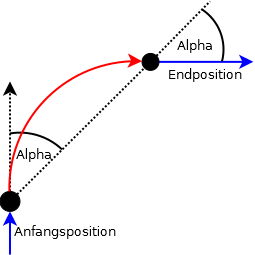
\includegraphics[scale=0.8]{Bilder/BerechnungOrientierung.png} 
\caption{Berechnung der Ausrichtung}
\end{figure}
Da das Auto im Vaterknoten N eine bestimmte Ausrichtung hat und mit nur einer Lenkeinstellung zum nächsten Knoten K gelangt, ist dort die Ausrichtung dadurch festgelegt und berechnet sich aus der Ausrichtung des Vaterknotens, Winkel $\theta$, und dem Winkel zwischen der Ausrichtung des Vaterknotens und dem Richtungsvektor von N nach K. Wie in der Zeichnung ~\ref{fig:fig8} zu sehen ist, berechnet sich die Ausrichtung $\omega$ des neuen Knotens K folgendermaßen:
\begin{center}
	$\theta + 2 \pi - 2*\alpha = \omega$
\end{center}

\subsubsection{Kostenfunktion}
\label{sec:Kosten}
Eine besondere Bedeutung zur Erzeugung einer "guten" Trajektorie kommt der Kostenfunktion zu. Diese sorgt nicht nur dafür, welcher Knoten als Vaterknoten ausgewählt wird, sondern spielt auch beim Neuverknüpfen des Baumes eine Rolle.Somit kann mithilfe der Kostenfunktion für besonders gut abfahrbare oder besonders kurze Pfade gesorgt werden. \\
Da durch die Orientierung des Vaterknotens die Orientierung des Kindknotens bereits festgelegt ist (siehe Abbildung ~\ref{fig:fig8}, können aus eigentlich geraden Strecken sehr ungünstige Pfade entstehen.\\
 In Abbildung ~\ref{fig:fig5} wird als Kostenfunktion der euklidische Abstand benutzt. Knoten C wählt aus B1 und B2 den nächsten Nachbarn aus, das ist B2. Leider entsteht dadurch eine sehr kurvige Route, bei der vom fast maximalem Lenkeinschlag nach rechts auf den maximalen Lenkeinschlag der anderen Seite gewechselt werden muss. Neben Nachteilen des Komforts, der Sicherheit und längerem Weg wird auch die Ungenauigkeit höher. Anfangs wurde angenommen, dass der Lenkwinkel sich sofort ändern kann. Während bei kleinen Änderungen diese Annahme nur für kleine Fehler sorgt, sind die Auswirkungen bei solch starken Änderungen deutlicher spürbar.


\begin{figure}[htb]
  \label{fig:fig6}  
    \centering
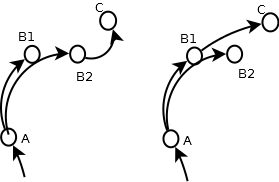
\includegraphics[scale=1]{Bilder/Gute_schlechte_funktion.png} 
\caption{Euklidische Kostenfunktion (rechts) gegenüber der erweiterten Kostenfunktion (links)}
\end{figure}


In Abbildung ~\ref{fig:fig9} hingegen wurde eine bessere Kostenfunktion gewählt, sodass über B1 gehend ein effizienterer, kürzerer Pfad entsteht. Die Kostenfunktion muss dabei die Ausrichtung des Autos beim Vaterknoten N berücksichtigen. \\
Es wurde eine Kombination aus dem euklidischem Abstand und der Winkeldifferenz der Knoten K und N zur Kostenberechnung zu benutzen. Die Kosten berechnen sich dann wie folgt: 
\begin{center}
$cost(K) = cost(N) +eukl. Abstand(K,N) * (1+Winkeldifferenz)$
\end{center} 
Bei einer geraden Strecke wird lediglich der euklidische Abstand als Kosten aufsummiert, bei einer Kehre von 180$^{\circ}$ bis zum vierfachen der euklidischen Kosten (Winkeldifferenz $\pi$ +1).\\
Nachteil dieser Kostenfunktion ist, dass nicht berücksichtigt wird, dass starke Kurven weniger schlimm sind auf größerer Strecke. Mit anderen Worten, das Fahren genau auf den minimalen Wendekreisen ist meist weniger angenehm beziehungsweise optimal als das Fahren auf weiten Kreisen, auch wenn beide Pfade die gleiche Winkeldifferenz haben. Das Problem hierbei ist, dass ein kleinerer Kreis geringere euklidische Kosten hat und demzufolge gegenüber dem größeren Kreis bevorzugt wird. Eine andere Möglichkeit wäre auch, die tatsächliche zu fahrende Strecke des Autos zu benutzen anstatt des euklidischen Abstands und dadurch effizientere Pfade zu bevorzugen. Eine andere Möglichkeit ist, zu harte Richtungsänderungen zu bestrafen und kleine $ \Delta \theta$ zu bevorzugen. \\
\subsubsection{Rewiring}
Der Knoten K wurde neu in den Baum hinzugefügt. Nun wird überprüft, ob bereits vorhandene Knoten besser erreichbar sind, wenn der Weg über K gewählt wird(siehe \ref{sec:rewiring}).
Dazu werden zunächst im Radius R alle in Frage kommenden Nachbarn ausgewählt. Diese Menge wird hier als M bezeichnet. Von M aussortiert werden alle, die entweder vom Knoten K aus nicht erreichbar sind (gleiche Überprüfungen wie in \ref{sec:Auswahl}) oder aber bei denen K keine Verbesserung bewirkt, also die Kosten - über den Knoten K - gleich oder höher sind). \\
\begin{figure}
\centering
\label{fig:rewiringNodeInvalid}
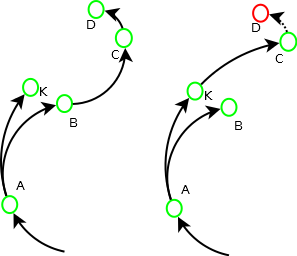
\includegraphics[scale=0.7]{Bilder/Rewiring_ungueltige_knoten.png} 
\caption{Knoten K wird neuer Nachbar von C - Knoten D kann nicht mehr erreicht werden}
\end{figure}

Wenn man allen in M enthaltenen Knoten einfach K als Vater hinzufügen würde, müsste jeweils die Orientierung der Knoten in M, der Winkel $\theta$, geändert werden. Das Auto gelangt auf anderem Wege zu diesen Knoten und hat somit eine andere Ausrichtung als vorher. Allerdings kann es dadurch vorkommen, dass wenn der Knoten $C \in M$ eine neue Orientierung hat, Kinder von C nicht mehr durch C erreichbar sind (siehe \ref{fig:rewiringNodeInvalid}). Deshalb wird, anstatt die Orientierung zu ändern, einfach ein neuer Knoten hinzugefügt, der zwar die gleicher Koordinaten hat wie C, aber eine andere Orientierung. Dies wird mit allen von K erreichbaren Knoten durchgeführt. Alle somit zum Baum neu hinzugefügten Knoten sind durch K besser erreichbar. Dadurch werden allerdings keine Pfade verbessert, was eine Voraussetzung für die in \ref{sec:rrt*} genannte asymptotische Optimalität ist.\\
Die einzige vollständige Maßnahme wäre, für jeden so neu hinzugefügten Knoten ebenfalls das Rewiring durchzuführen, da ein durch diesen Knoten andere eventuell durch bessere Pfade erreichbar ist. Dadurch braucht man jedoch sehr viel Zeit, da der ganze Baum z.T. mehrfach neu verknüpft wird. Im schlechtesten Fall wäre die Laufzeit dabei exponentiell, da jeder Knoten alle seine Nachbarn neu verknüpfen könnte.
\subsubsection{Bewertung}
Leider kann diese Herangehensweise nur zwei von den drei geforderten Anforderungen erreichen. Die Abfahrbarkeit der Trajektorie ist in jedem Fall gewährleistet. Die asymptotische Optimalität kann jedoch nur gewährleistet werden, wenn das Rewiring komplett durch den ganzen Baum rekursiv, das heißt auf jeden durch das Rewiring neu hinzugefügten Knoten, angewendet wird. Dadurch entstehen exponentielle Laufzeiten, sodass der Aufbau des Baumes mehrere Sekunden in Anspruch nimmt, was auch nach Optmierung des Codes und der Datenstruktur zu viel ist. [TODO Messwerte einfügen]\\
Deshalb ist dieser Ansatz für den produktiven Einsatz nicht geeignet.

\subsection{Zweiter Ansatz}
Auf dem ersten Ansatz aufbauend wurde der zweite entwickelt. Das Problem des ersten war, dass das Rewiring nicht richtig durchgeführt werden konnte, weil sonst Knoten ungültig werden. \\
Theoretisch kann aber ein Auto mit nur einer Lenkeinstellung alle Punkte außerhalb der Wendekreise erreichen. Das Problem der Nichterreichbarkeit könnte also dadurch behoben werden, dass nur Knoten in einem bestimmten Abstand - so dass sie nicht innerhalb der Wendekreise sind -als Vaterknoten erlaubt sind.\\
\begin{figure}
\centering
\label{fig:zweiteransatz}
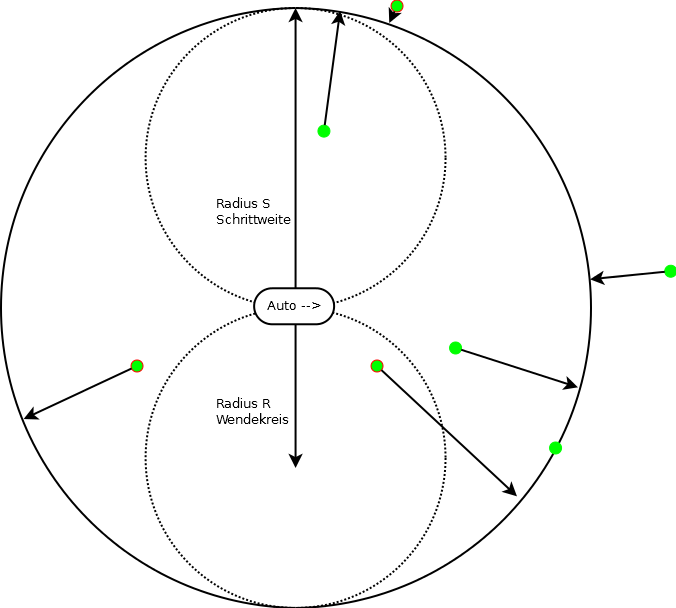
\includegraphics[scale=0.5]{Bilder/Zweiter_Ansatz_Projektion.png} 
\caption{Je nach dem, wo der Punkt erzeugt wurde, wird er auf Schrittweite verschoben}
\end{figure}
\subsubsection{Veränderungen}
Die im ersten Ansatz beschriebene Vorauswahl fällt weg, da erstmal jeder Knoten erreichbar ist. Bei der Projektion an den nächsten Nachbarn muss darauf geachtet werden, dass der Projektionsabstand größer als der Durchmesser der Wendekreise ist. Die Auswahl des Vaterknotens findet nur außerhalb eines bestimmten Kreises statt, da im Inneren je nach Ausrichtung des Autos nicht alle Punkte erreichbar sind. Der Radius des Kreises entspricht dem Durchmesser der Wendekreise des Autos (siehe \ref{fig:zweiteransatz}).\\
Dadurch gibt es keine ungültigen Punkte in der Trajektorie. Wenn das Rewiring durchgeführt wird, wird in allen Knoten, die durch den neu hinzugefügten Knoten besser erreichbar sind, die Ausrichtung neu berechnet, wie in \ref{sec:Rewiring} beschrieben. Als Kostenfunktion kann nur der euklidische Abstand verwendet werden, da die Ausrichtung veränderlich ist. \\
Die Abstände zwischen zwei so verbundenen Knoten sind sehr groß, was die Vermeidung von Hindernissen schwierig macht.\\
Auch können kurvige Trajektorien durch z.B. eine Kostenfunktion nicht vermieden werden, da die Kostenfunktion dazu die Ausrichtungen in einem Knoten benötigen würde, um die Änderung der Orientierung zu bestimmen. Diese Ausrichtungen können zwar bestimmt werde, ändern sich jedoch mit jeder Neuverknüpfung. Alle Kosten jedes Mal neu zu berechnen, würde mit O(n) viel zu lange dauern.\\
\subsubsection{Bewertung}
Wie beim ersten Ansatz ist die entstehende Trajektorie vom Auto abfahrbar, hat also keine unerreichbaren Knoten. Die Geschwindigkeit des Algorithmus hat sich im Gegensatz zum ersten Knoten stark verbessert und für die Rewiring Operation wird nur noch O(log n) Zeit benötigt. \\
Die Pfade können zwar durch das Rewiring optimiert werden, jedoch entstehen große Herausforderungen bei der Hindernisvermeidung. Außerdem können kleine Zielbereiche nur über Umwege erreicht werden, da sie sonst aufgrund der Schrittweite einfach übersprungen werden. Ein weiterer Nachteil ist, dass kurvige Trajektorien nicht aktiv vermieden werden, da die Kostenfunktion nur auf den Koordinaten der Knoten basieren kann. Somit sind beim Auto auf dem Weg zum Ziel Schlangenlinien zu erwarten und der Pfad ist in diesem Sinne nicht optimal [TODO durch Testergebnisse beweisen] 

\subsection{Dritter Ansatz}
Bei diesem Ansatz soll erst im Nachhinein ein abfahrbarer Pfad erzeugt werden. Dazu wird der RRT* Algorithmus ohne Berücksichtigung der Ausrichtung $\theta$ ausgeführt. Dadurch das keine Einschränkungen gemacht werden, terminiert der Algorithmus schnell. Zur Berechnung der Kosten eines jeden Knoten wird eine Kostenfunktion c(K) verwendet. Sei K ein Knoten und V der Vater dieses Knotens: 
$c(K) = c(V) + euklid. dist(K,V)$   \\
\subsubsection{Erzeugung der Trajektorie}
Es wird der Zielknoten Z ausgewählt. Für diesen Knoten Z wird die Menge M aller Knoten in einem Kreis um Z gebildet.  Aus der Menge M wird der Vaterknoten V bestimmt, dessen Gesamtkosten am geringsten ist. Dabei wird zur Berechnung der Gesamtkosten auch die Änderung der Ausrichtung, um zu diesem Zielknoten zu gelangen, berücksichtigt, ähnlich wie in der Kostenfunktion des ersten Ansatzes. \\
Nach einer Laufzeit von maximal O(n log n) ist der Startknoten erreicht. Dadurch, dass vom Zielknoten aus gestartet wurde, kann es sein, dass das Auto vom Startknoten aus den ersten Knoten der Trajektorie gar nicht oder nicht mit der richtigen Orientierung erreichen kann. Deshalb werden für den ersten Schritt Dubins curves verwendet, mit denen das Auto einen beliebigen Punkt mit beliebiger Ausrichtung erreichen kann. Nach diesem ersten Schritt kann das Auto jeden Knoten mit nur einer Lenkeinstellung erreichen. \\

\subsubsection{Bewertung}
Durch RRT* und die Kostenfunktionen wird durch diesen Algorithmus nicht nur eine gültige Trajektorie erzeugt, sondern auch eine, bei der unnötige Kurven vermieden werden. Die Laufzeit liegt mit O(n log n) in einem vertretbaren Rahmen. \\
Bei der Problembeschreibung (\ref{sec:uebersicht}) wurde festgesetzt, dass der Algorithmus mindestens vier Mal pro Sekunde durchgeführt werden soll. Es ist zu erwarten, dass das Auto mehr als 250 Millisekunden braucht, um auf den vorgeschlagenen Pfad zu kommen, also den ersten Knoten mit korrekter Ausrichtung zu erreichen. Nach 250 Millisekunden wird jedoch ein komplett neuer Baum aufgebaut, sodass alle aufwändigen Berechnungen, um eine gute Trajektorie zu erstellen, umsonst waren. Somit wird das Auto stets nur den ersten Teil mit den Dubins curves abfahren, was den ganzen Sinn des Algorithmus in Frage stellt. \\
Dieser Ansatz ist also so ausgeführt nicht sinnvoll. Eine Möglichkeit wäre, den Baum wiederzuverwenden und somit auch die erzeugte Trajektorie. Allerdings muss dafür die Datenstruktur das sogenannte Prunning, also Abtrennen von Ästen des Baumes, unterstützen, um keine nicht erreichbaren Knoten und deren Kinder zu verwenden. Ohne diese Datenstruktur ist ein weiteres Vertiefen in diesen Ansatz nicht sinnvoll.

\subsection{Vierter Ansatz}
Nach dem erfolglosen Beschäftigen mit dem dritten Ansatz wurde der Fokus wieder mehr auf den ursprünglichen Ansatz und das Rewiring gelegt. Ziel war es nun, anstelle des rekursiven Rewiring eine andere, schnellere und trotzdem asymptotisch optimale Lösung zu finden. \\
\subsubsection{Rewiring}
Das Problem war, das mit jedem Rewiring eine große Anzahl an Knoten hinzugefügt wurden, auch wenn diese zum Teil nur marginale Verbesserungen boten, und dass jeder so hinzugefügte Knoten jeweils auch eine Rewiring Operation auslöste.\\
Anstatt für jeden Knoten, der durch das Rewiring besser erreichbar ist, einen neuen Knoten hinzuzufügen (\ref{sec:rewiring}) wird nur dem Knoten K ein neuer Knoten hinzugefügt, bei dem die Auswirkungen am größten sind. Dazu werden die Kosten von K mit den Kosten verglichen, die ein neu hinzugefügter Knoten an der Position von K hätte. Dies wird mit allen Knoten im Radius R durchgeführt und beim Paar mit der größten Differenz wird tatsächlich ein neuer Knoten hinzugefügt. \\
\begin{figure}
\label{fig:rewiring4}
\centering
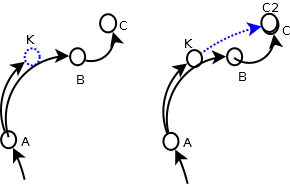
\includegraphics[scale=1]{Bilder/Rewiring.png} 
\caption{Rewiring}
\end{figure}
Das Ganze wird verdeutlicht an einem Beispiel in \ref{fig:rewiring4}. Hier wird Knoten K neu hinzugefügt. In der Liste der Erreichbaren Knoten stehen B und C. Weil bei B keine Kostenverbesserung stattfindet, ist bei C die Differenz zwischen alten Kosten und Kosten eines neuen Knotens an dieser Position am geringsten. Deshalb wird nun mit den gleichen Koordinaten wie C ein neuer Knoten $C_2$ erstellt. Nun wird überprüft ob $C_2$ weitere Knoten verbessern kann. Da dies nicht der Fall ist, endet das Rewiring und der Algorithmus fährt normal fort.\\
Das Rewiring wird so lange durchgeführt, bis kein Knoten mehr gefunden wird, dessen Kosten durch Neuverknüpfung geringer wären. Bei einer geeigneten Wahl der Schrittweite (nicht zu groß, \ref{sec:Auswahl}) kann dies relativ schnell eintreten, weil gar nicht so viele in Frage kommen. \\
Damit nicht immer beim gleichen Knoten das Rewiring durchgeführt wird, weil die Kostendifferenz bei diesem Knoten immer am höchsten ist, werden im alten Knoten auch die Kosten des neuen Knotens, der die gleichen Koordinaten hat, gespeichert. Beim Rewiring wird ein Knoten mit diesen Koordinaten nur dann hinzugefügt, falls dessen Kosten geringer sind als die aller Knoten mit diesen Koordinaten.

\subsubsection{Bewertung}
Der Vorteil dieses Mechanismus ist, dass mögliche Optimierungen schnell durch den Baum wandern und keine Knoten ungültig werden. Außerdem müssen nicht so viele randomisierte Punkte erzeut werden, was der Laufzeit zu Gute kommt.\\
 Nachteile sind allerdings eine geringere Anzahl von räumlich verteilten Punkten (es liegen Punkte \glqq übereinander\grqq). Zudem kann dieses Verfahren viel Zeit beanspruchen, ohne viel Effekt zu haben, wenn bereits viele Punkte im Baum existieren und Bereiche weit abseits der Zielregion neu verknüpft werden. \\
 Abschließend kann man sagen, dass von allen vier Ansätzen dieser der vielversprechenste ist. Es werden nicht nur gültige Pfade gefunden, sondern auch optimale, die in angemessener Zeit berechnet werden können[TODO Testergebnisse/Beweis].


\subsection{Dokumentation der Durchführung und Erkenntnisse daraus}
[TODO - mit rein nehmen oder rauslassen?] 



\subsubsection{Beschreibung erkannter Schwierigkeiten und Fehler}
[TODO - mit rein nehmen oder rauslassen?] 
Im Nachhinein betrachtet habe ich viele methodische Fehler gemacht. Zuerst wurde das Problem begutachtet, dann analysiert und ein Lösungsvorschlag gemacht. Dieser Lösungsvorschlag wurde aber nicht bis ins Detail auf die Machbarkeit überprüft, sondern ich habe versucht Teile davon direkt umzusetzen. Insgesamt habe ich den Aufwand dieser ersten Umsetzung stark unterschätzt. Ich musste mich sowohl in eine unbekannte Programmiersprache (C++) und in ein weitgehend unbekanntes Framework (ROS) einarbeiten. Besonders bei Letzterem kommunizierte ich zu wenig mit den wissenschaftlichen Mitarbeitern des Arbeitsbereichs. Somit verschlang schon die Einarbeitung und der Entwurf eines Prototypens sehr viel Zeit, ohne zu befriedigenden Ergebnissen zu kommen. Doch auch technische Probleme und Schwierigkeiten mit der vorhandenen Infrastruktur nahmen viel Zeit in Anspruch.\\
Als der Lösungsansatz endlich vollständig implementiert wurde, ist aufgefallen, dass dieser an einigen Stellen nicht funktionierte. Deshalb wurde versucht, den Lösungsansatz zu verbessern und diese verbesserte Lösung zu implementieren. Da ich zu wenig dabei mit anderen Mitarbeitern kommunizierte, hatte auch die verbesserten Lösungen Fehler, sodass ich mich oft in Sackgassen wiederfand. \\
Besonders am Anfang war, kombiniert mit häufigem Scheitern an Abhängigkeiten und Installationsproblemen, die dadurch resultierende Motivationslosigkeit ein großes Problem, was dann auch schnell zu einem Zeitproblem wurde. 

\subsubsection{Verbesserungen in der Arbeitsweise}
Ich habe festgestellt, dass sowohl detallierte Planung (was mache ich an jedem Tag der nächsten Woche) als auch globale Planung (welche Artefakte sollen bis wann fertig gestellt werden?) sehr wichtig sind und gründlich mit Sorgfalt durchgeführt werden sollten. \\
Bei Fehlschlägen ist es wichtig, sich - je nach Problem - an andere zu wenden, wenn man selbst das Problem nicht ohne weiteres lösen kann. Dies ist vor allem bei wiederkehrenden Problemen wie beim Aufsetzen von Software der Fall, deren Lösung längst bekannt ist. \\
Es ist sehr wichtig, sich über den theoretischen Ansatz und dessen Machbarkeit intensiv Gedanken zu machen, dabei auch verschiedene wissenschaftliche Quellen zu untersuchen. Stellt sich heraus, dass der eigene Ansatz nicht umsetzbar ist, sollte ein Gespräch mit dem Betreuer vereinbart werden, um Lösungen zu besprechen, bevor eigene fehlerhafte Ansätze implementiert werden. \\
Bei den Gesprächen mit den Mitarbeitern und Betreuern ist es wichtig, ein klares Anliegen bzw. eine klare Problemstellung zu haben und dies angemessen zu formulieren.

% !TeX encoding = UTF-8
\section{Zusammenfassung}
\label{Zusammenfassung}
...


\bibliography{bibliography}

\appendix
% !TeX encoding = UTF-8
\section{Anhang}

Quellcode der \LaTeX-Klasse \texttt{agse-thesis}:\footnote{Es ist nicht üblich,
den gesamten produzierten Quellcode bei einer Abschlussarbeit in Textform
abzugeben.}

\lstinputlisting[
    language={[LaTeX]Tex},
    morekeywords={ProvidesClass, DeclareOption, PassOptionsToClass,
        ProcessOptions, CurrentOption, LoadClass, RequirePackage, ifthenelse,
        ifcsdef, equal, definecolor, lstset, pgfkeys},
    basicstyle=\footnotesize\ttfamily,
    numbers=left,
    numberstyle=\footnotesize\ttfamily,
    stepnumber=5,
    inputencoding=utf8,
    extendedchars=true,
   literate={ä}{{\"a}}1 {ü}{{\"u}}1,
]{agse-thesis.cls}


\end{document}
